\documentclass[tikz]{standalone}

\begin{document}
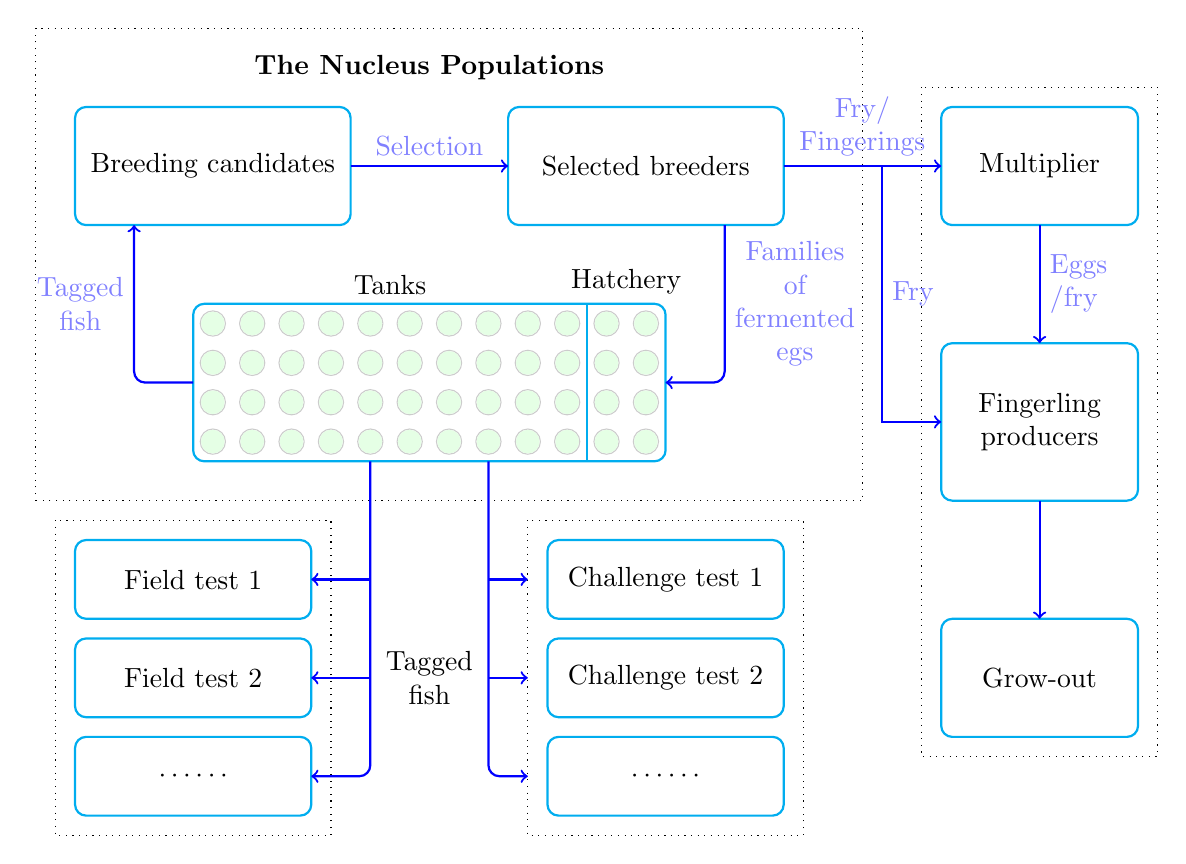
\begin{tikzpicture}
  % The nucleus part
  \draw [dotted] (0,0) rectangle (10.5,6);
  \node at (5,5.5) {\textbf{The Nucleus Populations}};
  %\draw [help lines] (0,0) grid (10.5, 6);
  \draw [thick, cyan, rounded corners] (0.5, 5) rectangle (4, 3.5);
  \draw [thick, cyan, rounded corners] (6, 5) rectangle (9.5, 3.5);
  \node at (2.25, 4.25) {Breeding candidates};
  \node at (7.75, 4.25) {Selected breeders};
  \draw [->, thick, blue] (4, 4.25) --node[above,blue!50]{Selection} (6, 4.25);
  \draw [cyan, thick, rounded corners] (2, 0.5) rectangle (8, 2.5);
  \draw [cyan, thick] (7, 0.5) -- (7, 2.5);
  \node [above] at (4.5, 2.5){Tanks};
  \node [above] at (7.5, 2.5){Hatchery};
  \draw [blue, rounded corners, ->, thick] (2, 1.5)--(1.25, 1.5)--node[left,align=center,blue!50]{Tagged\\fish}(1.25, 3.5);
  \draw [blue, rounded corners, ->, thick] (8.75, 3.5)--node[right, align=center, blue!50]{Families\\of\\fermented\\egs}(8.75, 1.5)--(8,1.5);
  % tanks
  \foreach \x in {2.25, 2.75,...,7.75}
  \foreach \y in {0.75,1.25,1.75,2.25}
  {
    \draw[gray!40](\x,\y) circle(0.16);
    \fill[green!10](\x,\y) circle(0.15);
  }
  % the field test block
  \draw [dotted] (0.25, -0.25) rectangle (3.75, -4.25);
  \draw [thick, cyan, rounded corners] (0.5, -0.5) rectangle (3.5, -1.5);
  \node at (2, -1) {Field test 1};
  \draw [thick, cyan, rounded corners] (0.5, -1.75) rectangle (3.5, -2.75);
  \node at (2, -2.25) {Field test 2};
  \draw [thick, cyan, rounded corners] (0.5, -3) rectangle (3.5, -4);
  \node at (2, -3.5) {$\cdots\cdots$};
  % The challege block
  \draw [dotted] (6.25, -0.25) rectangle (9.75, -4.25);
  \draw [thick, cyan, rounded corners] (6.5, -0.5) rectangle (9.5, -1.5);
  \node at (8, -1) {Challenge test 1};
  \draw [thick, cyan, rounded corners] (6.5, -1.75) rectangle (9.5, -2.75);
  \node at (8, -2.25) {Challenge test 2};
  \draw [thick, cyan, rounded corners] (6.5, -3) rectangle (9.5, -4);
  \node at (8, -3.5) {$\cdots\cdots$};
  \node [align=center] at (5, -2.25) {Tagged\\fish};
  % Connections between nucleus and fields
  \draw [blue, rounded corners, thick, ->](4.25, 0.5)--(4.25, -3.5)--(3.5, -3.5);
  \draw [blue, thick, ->](4.25, -2.25)--(3.5, -2.25);
  \draw [blue, thick, ->](4.25, -1) --(3.5, -1);
  % Connections between nucleus and challenges
  \draw [blue, rounded corners, thick, ->](5.75, 0.5)--(5.75, -3.5)--(6.25, -3.5);
  \draw [blue, thick, ->](5.75, -2.25)--(6.25, -2.25);
  \draw [blue, thick, ->](5.75, -1) --(6.25, -1);
  % The production part
  \draw [dotted] (11.25, 5.25) rectangle (14.25, -3.25);
  \draw [cyan, thick, rounded corners] (11.5,5) rectangle (14, 3.5);
  \node at (12.75, 4.25){Multiplier};
  \draw [cyan, thick, rounded corners] (11.5,2) rectangle (14, 0);
  \node[align=center] at (12.75, 1){Fingerling\\producers};
  \draw [cyan, thick, rounded corners] (11.5, -1.5) rectangle (14, -3);
  \node at (12.75, -2.25){Grow-out};
  \draw [->,blue,thick](12.75, 3.5) --node[right,align=left, blue!50]{Eggs\\/fry}(12.75, 2);
  \draw [->,blue,thick](12.75, 0) -- (12.75, -1.5);
  % Connections between nucleus and production
  \draw [->,blue,thick](9.5,4.25)--node[above,align=center, blue!50]{Fry/\\Fingerings}(11.5,4.25);
  \draw [->,blue,thick](10.75,4.25)--node[right, blue!50]{Fry}(10.75,1)--(11.5,1);
\end{tikzpicture}
\end{document}
